\documentclass[11pt]{report}
\usepackage[a4paper]{geometry}
\usepackage[myheadings]{fullpage}
\usepackage{fancyhdr}
\usepackage{lastpage}
\usepackage{graphicx, wrapfig, subcaption, setspace, booktabs}
\usepackage[T1]{fontenc}
\usepackage[font=small, labelfont=bf]{caption}
\usepackage[protrusion=true, expansion=true]{microtype}
\usepackage{sectsty}
\usepackage{url, lipsum}
\usepackage{mathptmx}
\usepackage[utf8]{inputenc}
\usepackage[francais]{babel}
\pagestyle{plain}

\newcommand{\HRule}[1]{\rule{\linewidth}{#1}}
\onehalfspacing
\setcounter{tocdepth}{5}
\setcounter{secnumdepth}{5}

\renewcommand{\thesection}{\arabic{section}}

%-------------------------------------------------------------------------------
% TODO
%-------------------------------------------------------------------------------

%% Améliorer le cahier des charges pour la semaine prochaine.


%-------------------------------------------------------------------------------
% TITLE PAGE
%-------------------------------------------------------------------------------

\begin{document}

\title
{
	\Large{Cahier des charges}
	\HRule{2pt} \\ [0.5cm]
	\LARGE \textbf{\uppercase{Bacchanight}}
	\HRule{2pt} \\ [0.5cm]
	\normalsize \today
}

\date{}

\author
{
	\LARGE{Université de Bordeaux} \\
	\\
	Alexandre CASANOVA FRANGER \\
	Guillaume CHARLET \\
    Kenji FONTAINE \\
    Gauthier LAMARQUE \\
	Ny Andry RAHARISON \\
}

\maketitle

%-------------------------------------------------------------------------------
% Présentation du projet + Besoins fonctionnels
%-------------------------------------------------------------------------------

\renewcommand{\thesection}{\arabic{section}}

\section{Présentation}

La Baccanight est une soirée organisée par le Musée des Beaux Arts de Bordeaux.
Elle a pour but de mettre en avant le musée et ses oeuvres à un publique plus jeune.
Le but de ce projet est d'élaborer un outil permettant de mieux renseigner les internautes.

\section{Besoins fonctionnels}

Le site doit utiliser le même système de gestion du contenu que le site actuel
du musée des beaux arts : \textbf{Drupal 7}. \\

Le site doit permettre l'accès aux informations suivantes :
\begin{itemize}
	\item Description de la soirée (date et lieu).
	\item Programme/Planning de la soirée.
	\item Historique des sessions précédentes.
	\item Plan d'accès Google Maps.
	\item Contact, lien vers les réseaux sociaux du Musée des Beaux Arts.
\end{itemize}

L'ensemble des informations ci-dessus doit être modifiable par une personne
ayant accès au CMS Drupal. \\
%% Détailler, comment, facile ? difficile ?, mise en page ou pas ? Avoir à coder
%% ou pas ?
%% Donner le moins possible de contrôle à l'utilisateur.
%%


\subsection*{Hébergement}
Prise de contact avec la Mairie de Bordeaux, actuellement chargée de
l'hébergement du site du Musée des Beaux-Arts.

\subsection*{Déploiement}
Création de la page en utilisant le système de gestion de contenu Drupal
(version 7) déjà présent sur le site du Musée des Beaux-Arts.
Un manuel permettant à une personne ayant de l'expérience avec Drupal
d'intégrer le site au site actuel du musée devra être fourni.

%-------------------------------------------------------------------------------
% Besoins non fonctionnels
%-------------------------------------------------------------------------------

\newpage

\section{Besoins non fonctionnels}

\subsection*{Charte graphique}

Le site doit respecter le code couleur de la soirée :
%% Les couleurs doivent être modifiables par le user.
\begin{itemize}
	\item mauve (\#e37fff)
	\item rose  (\#f213a4)
\end{itemize}

Le site est sous un format One Page. Un site One Page est un site constitué
d'une seule et même page sur laquelle l'ensemble des informations du site web
est disponible en scrollant (ou à l'aide d'une barre de navigation).

\subsection*{Accessibilité}

Le site doit être accessible à partir des navigateurs pour ordinateur
couramment utilisés :
%% Ajouter les numéros de versions.
\begin{itemize}
	\item Google Chrome
	\item Mozilla Firefox
	\item Internet Explorer
	\item Safari
	\item Opera
\end{itemize}

Le site doit être accessible à partir des navigateurs pour smartphone
couramment utilisés :
\begin{itemize}
	\item Safari
	\item Google Chrome
	\item Mozilla Firefox
\end{itemize}

\subsection*{Responsive}
Le site doit s'adapter à la taille de l'écran.

\subsection*{Léger}
Le site doit se charger en moins de X secondes, en utilisant une connection à
X ko/s.

%-------------------------------------------------------------------------------
% Retro planning
%-------------------------------------------------------------------------------

Version statique pour le 21 Mars.
%% Créer un nouveau dépôt
%% Fixer des priorités.
%% Préciser les versions etc...
%% Contrainte d'accessibilité
%% Compléter le retro planning
%% Qu'est-ce qu'on pourrait faire avec plus de temps, argent, moyen etc...
%% Faire le retro planning
%% Diagramme de Gantt
%% github : GuillaumeBlin

%-------------------------------------------------------------------------------
% Maquette
%-------------------------------------------------------------------------------

\newpage

\section{Annexe : Maquette}

\vspace{0.4cm}
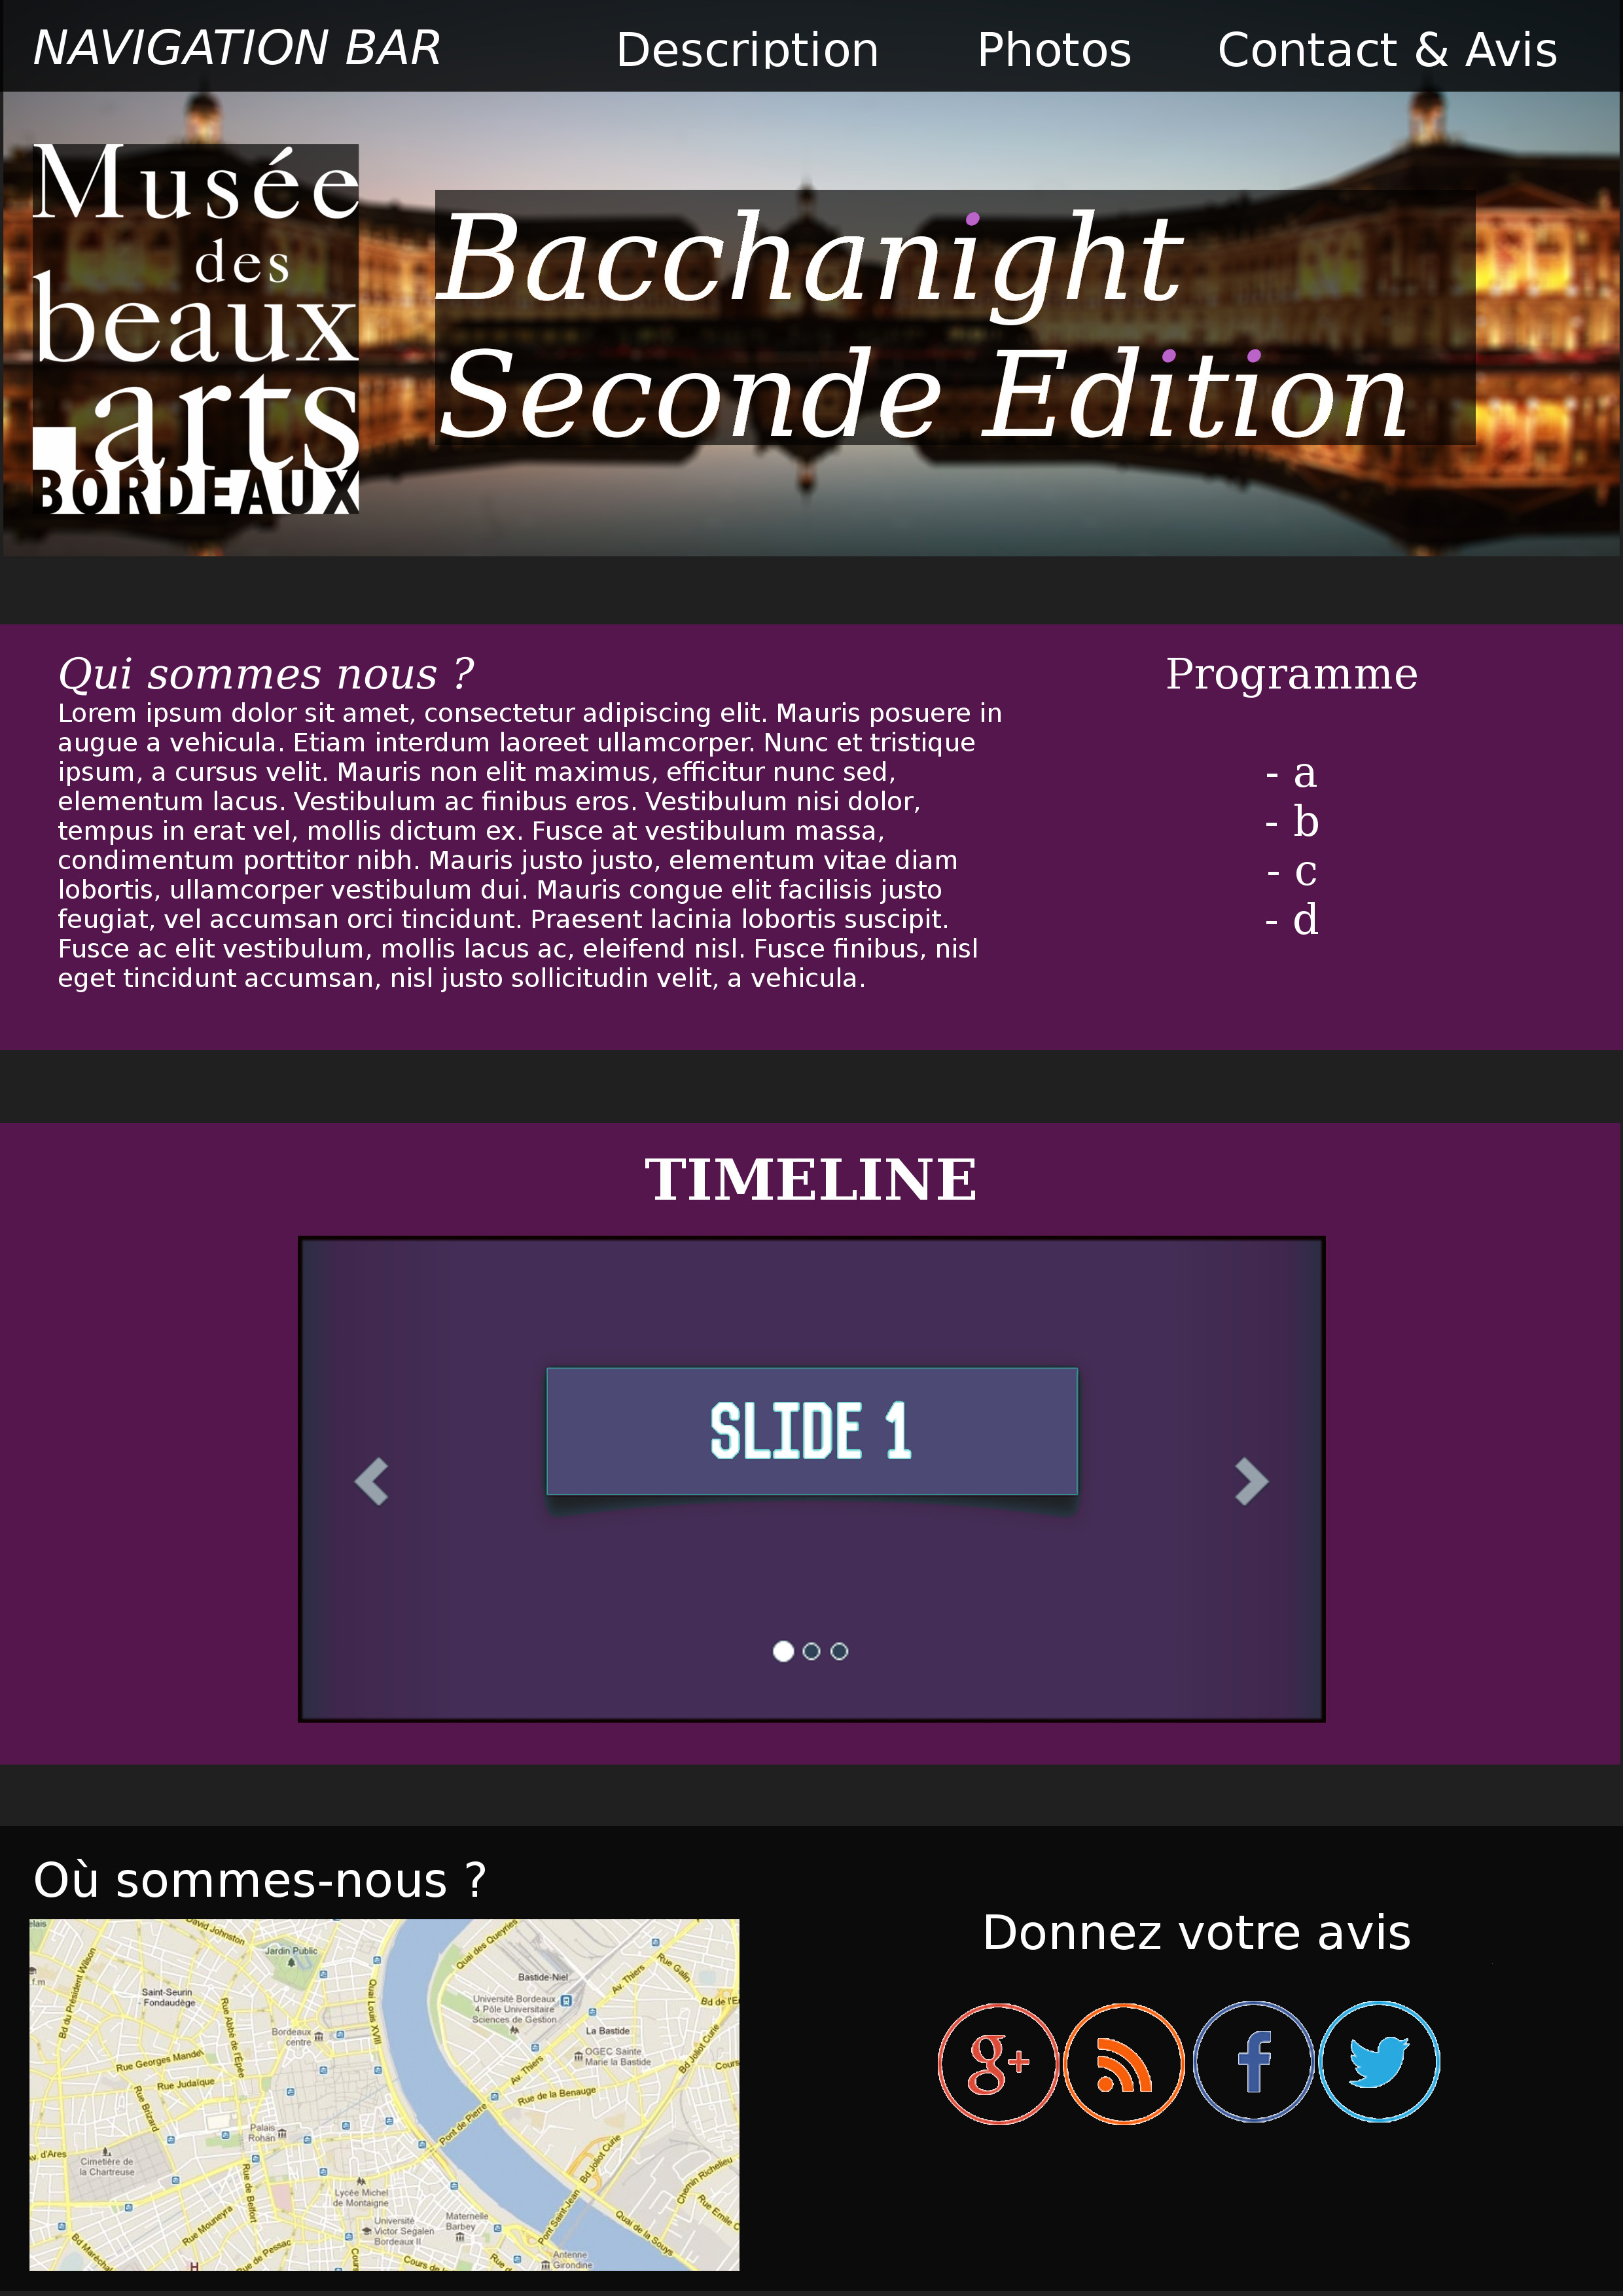
\includegraphics[scale=0.75]{maquette.jpg}

\end{document}
